\documentclass[a4paper]{book}
\usepackage{makeidx}
\usepackage{graphicx}
\usepackage{multicol}
\usepackage{float}
\usepackage{listings}
\usepackage{color}
\usepackage{textcomp}
\usepackage{alltt}
\usepackage{times}
\usepackage{ifpdf}
\ifpdf
\usepackage[pdftex,
            pagebackref=true,
            colorlinks=true,
            linkcolor=blue,
            unicode
           ]{hyperref}
\else
\usepackage[ps2pdf,
            pagebackref=true,
            colorlinks=true,
            linkcolor=blue,
            unicode
           ]{hyperref}
\usepackage{pspicture}
\fi
\usepackage[utf8]{inputenc}
\usepackage{doxygen}
\lstset{language=C++,inputencoding=utf8,basicstyle=\footnotesize,breaklines=true,breakatwhitespace=true,tabsize=8,numbers=left }
\makeindex
\setcounter{tocdepth}{3}
\renewcommand{\footrulewidth}{0.4pt}
\begin{document}
\hypersetup{pageanchor=false}
\begin{titlepage}
\vspace*{7cm}
\begin{center}
{\Large Diff2D }\\
\vspace*{1cm}
{\large Generated by Doxygen 1.6.1}\\
\vspace*{0.5cm}
{\small Tue May 27 11:41:57 2014}\\
\end{center}
\end{titlepage}
\clearemptydoublepage
\pagenumbering{roman}
\tableofcontents
\clearemptydoublepage
\pagenumbering{arabic}
\hypersetup{pageanchor=true}
\chapter{Module Index}
\section{Modules}
Here is a list of all modules:\begin{DoxyCompactList}
\item \contentsline{section}{Core}{\pageref{group__group__core}}{}
\end{DoxyCompactList}

\chapter{Class Index}
\section{Class Hierarchy}
This inheritance list is sorted roughly, but not completely, alphabetically\-:\begin{DoxyCompactList}
\item \contentsline{section}{\-\_\-\-\_\-array$<$ T, N $>$}{\pageref{class____array}}{}
\item \contentsline{section}{\-\_\-\-\_\-multivec$<$ D, U $>$}{\pageref{struct____multivec}}{}
\item \contentsline{section}{\-\_\-\-\_\-multivec$<$ 1, U $>$}{\pageref{struct____multivec_3_011_00_01U_01_4}}{}
\item \contentsline{section}{Conn}{\pageref{classConn}}{}
\item \contentsline{section}{Equation}{\pageref{classEquation}}{}
\item \contentsline{section}{Equation\-\_\-\-Prob}{\pageref{classEquation__Prob}}{}
\item \contentsline{section}{Index\-\_\-\-Lambda}{\pageref{structIndex__Lambda}}{}
\item \contentsline{section}{Initializer\-\_\-list$<$ D, U $>$}{\pageref{structInitializer__list}}{}
\item \contentsline{section}{Initializer\-\_\-list$<$ 1, U $>$}{\pageref{structInitializer__list_3_011_00_01U_01_4}}{}
\item \contentsline{section}{I\-S}{\pageref{structIS}}{}
\item \contentsline{section}{Local\-Coor}{\pageref{classLocalCoor}}{}
\begin{DoxyCompactList}
\item \contentsline{section}{Face}{\pageref{classFace}}{}
\item \contentsline{section}{Patch}{\pageref{classPatch}}{}
\end{DoxyCompactList}
\item \contentsline{section}{Patch\-\_\-\-Group}{\pageref{classPatch__Group}}{}
\item \contentsline{section}{Prob}{\pageref{classProb}}{}
\item \contentsline{section}{Term}{\pageref{structTerm}}{}
\end{DoxyCompactList}

\chapter{Class Index}
\section{Class List}
Here are the classes, structs, unions and interfaces with brief descriptions\-:\begin{DoxyCompactList}
\item\contentsline{section}{\hyperlink{class____array}{\-\_\-\-\_\-array$<$ T, N $>$} }{\pageref{class____array}}{}
\item\contentsline{section}{\hyperlink{struct____multivec}{\-\_\-\-\_\-multivec$<$ D, U $>$} }{\pageref{struct____multivec}}{}
\item\contentsline{section}{\hyperlink{struct____multivec_3_011_00_01U_01_4}{\-\_\-\-\_\-multivec$<$ 1, U $>$} }{\pageref{struct____multivec_3_011_00_01U_01_4}}{}
\item\contentsline{section}{\hyperlink{classConn}{Conn} }{\pageref{classConn}}{}
\item\contentsline{section}{\hyperlink{classEquation}{Equation} }{\pageref{classEquation}}{}
\item\contentsline{section}{\hyperlink{classEquation__Prob}{Equation\-\_\-\-Prob} }{\pageref{classEquation__Prob}}{}
\item\contentsline{section}{\hyperlink{classFace}{Face} }{\pageref{classFace}}{}
\item\contentsline{section}{\hyperlink{structIndex__Lambda}{Index\-\_\-\-Lambda} }{\pageref{structIndex__Lambda}}{}
\item\contentsline{section}{\hyperlink{structInitializer__list}{Initializer\-\_\-list$<$ D, U $>$} }{\pageref{structInitializer__list}}{}
\item\contentsline{section}{\hyperlink{structInitializer__list_3_011_00_01U_01_4}{Initializer\-\_\-list$<$ 1, U $>$} }{\pageref{structInitializer__list_3_011_00_01U_01_4}}{}
\item\contentsline{section}{\hyperlink{structIS}{I\-S} }{\pageref{structIS}}{}
\item\contentsline{section}{\hyperlink{classLocalCoor}{Local\-Coor} }{\pageref{classLocalCoor}}{}
\item\contentsline{section}{\hyperlink{classPatch}{Patch} }{\pageref{classPatch}}{}
\item\contentsline{section}{\hyperlink{classPatch__Group}{Patch\-\_\-\-Group} }{\pageref{classPatch__Group}}{}
\item\contentsline{section}{\hyperlink{classProb}{Prob} }{\pageref{classProb}}{}
\item\contentsline{section}{\hyperlink{structTerm}{Term} }{\pageref{structTerm}}{}
\end{DoxyCompactList}

\chapter{Module Documentation}
\hypertarget{group__group__core}{
\section{Core}
\label{group__group__core}\index{Core@{Core}}
}
\subsection*{Classes}
\begin{DoxyCompactItemize}
\item 
class \hyperlink{classProb}{Prob}
\begin{DoxyCompactList}\small\item\em Problem \item\end{DoxyCompactList}\end{DoxyCompactItemize}


\subsection{Detailed Description}
This group contains core objects 
\chapter{Class Documentation}
\hypertarget{class____array}{
\section{\_\-\_\-array$<$ T, N $>$ Class Template Reference}
\label{class____array}\index{\_\-\_\-array@{\_\-\_\-array}}
}
Collaboration diagram for \_\-\_\-array$<$ T, N $>$:\nopagebreak
\begin{figure}[H]
\begin{center}
\leavevmode
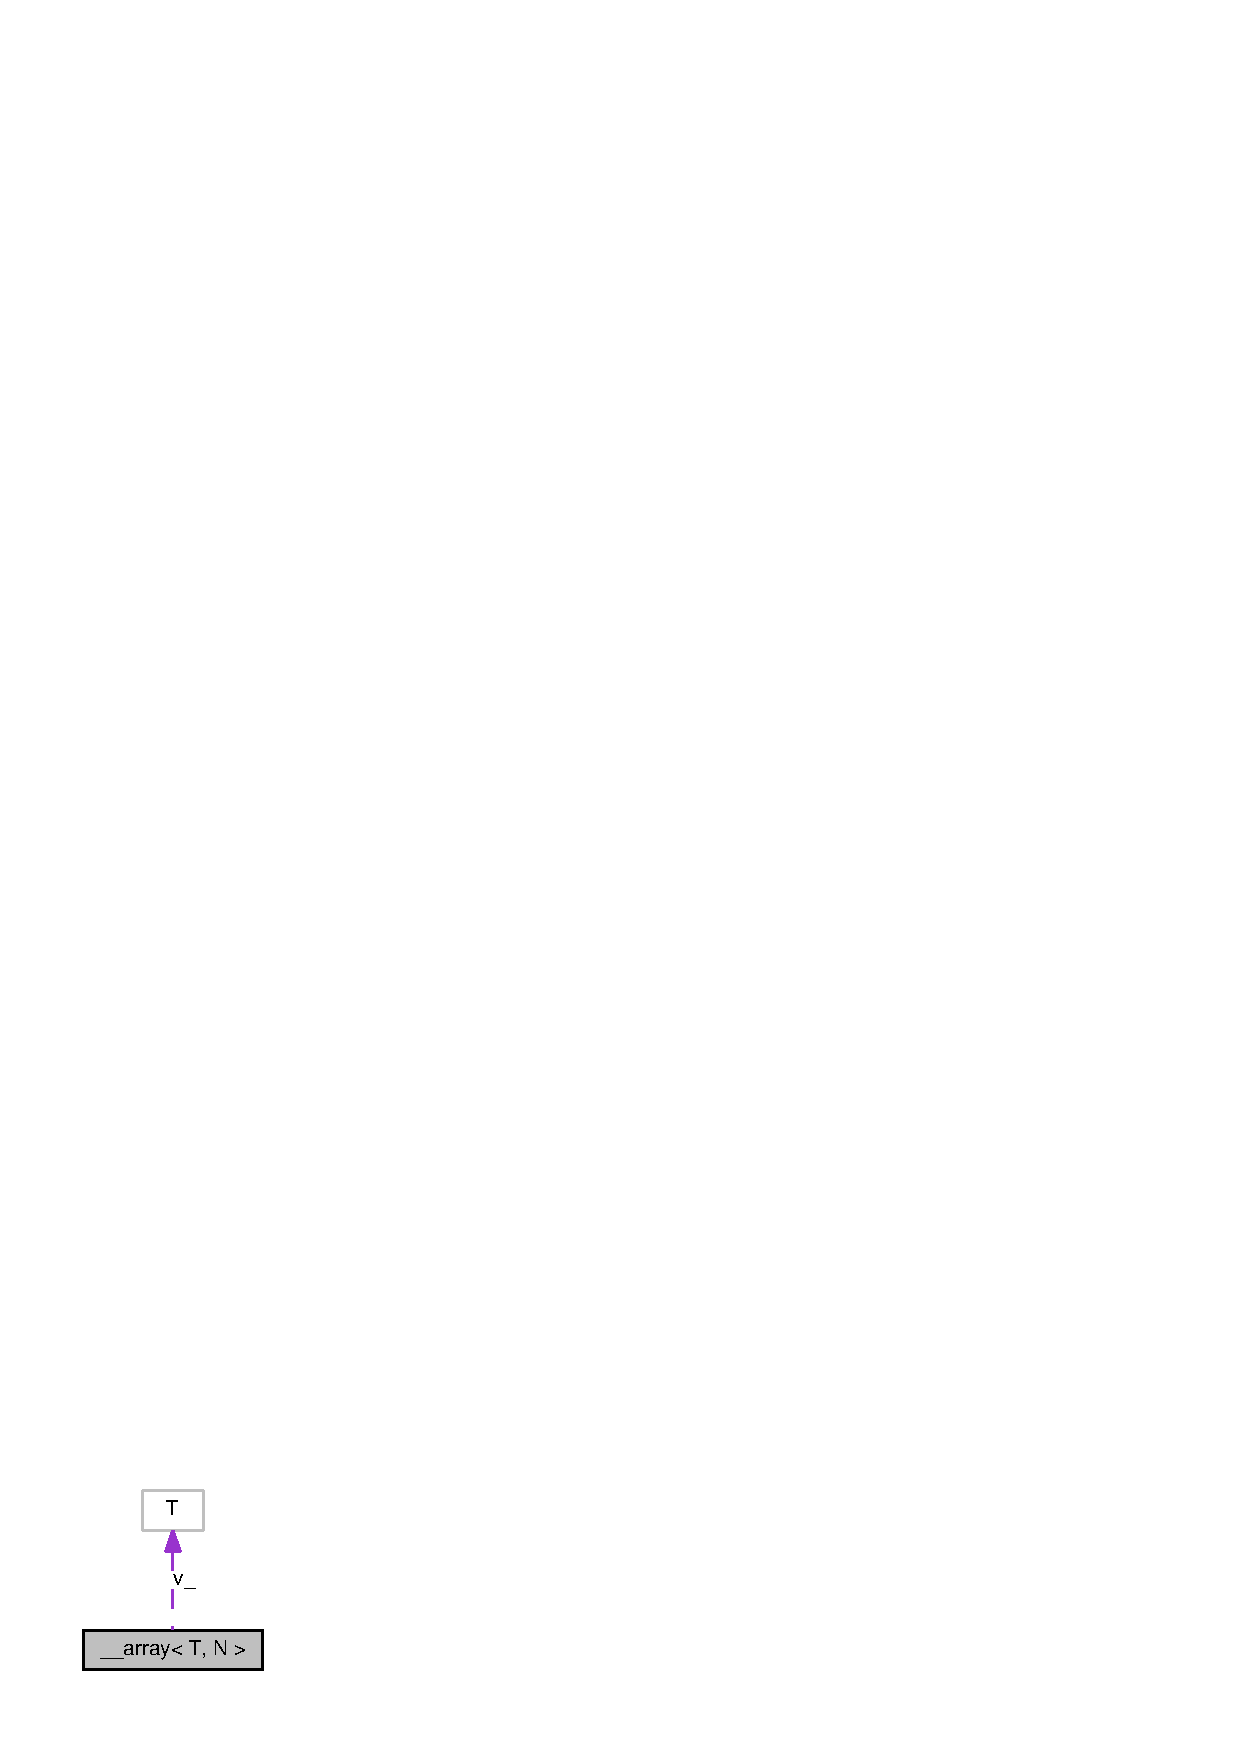
\includegraphics[width=130pt]{class____array__coll__graph}
\end{center}
\end{figure}
\subsection*{Public Types}
\begin{DoxyCompactItemize}
\item 
\hypertarget{class____array_a90230a0abce0d451b9425b69b24534e5}{
typedef std::shared\_\-ptr$<$ \hyperlink{class____array}{\_\-\_\-array}$<$ T, N $>$ $>$ {\bfseries shared}}
\label{class____array_a90230a0abce0d451b9425b69b24534e5}

\item 
\hypertarget{class____array_ab58bead881f51e40d3fb088e8adb2d77}{
typedef \hyperlink{structInitializer__list}{Initializer\_\-list}$<$ N, T $>$::list\_\-type {\bfseries init\_\-list}}
\label{class____array_ab58bead881f51e40d3fb088e8adb2d77}

\end{DoxyCompactItemize}
\subsection*{Public Member Functions}
\begin{DoxyCompactItemize}
\item 
\hypertarget{class____array_ac3443fee161fd3f8ccb1290980a4190d}{
{\bfseries \_\-\_\-array} (\hyperlink{class____array}{\_\-\_\-array}$<$ T, N $>$ const \&rhs)}
\label{class____array_ac3443fee161fd3f8ccb1290980a4190d}

\item 
\hypertarget{class____array_a1072f5c538102121515000a4ef521303}{
void {\bfseries zeros} ()}
\label{class____array_a1072f5c538102121515000a4ef521303}

\item 
\hypertarget{class____array_ad1fd7d5c46fb341f54cab916b78be561}{
void {\bfseries ones} ()}
\label{class____array_ad1fd7d5c46fb341f54cab916b78be561}

\item 
\hypertarget{class____array_ae6a7f942aeb5857504e9db83f7cfac57}{
void {\bfseries set} (std::initializer\_\-list$<$ T $>$ src)}
\label{class____array_ae6a7f942aeb5857504e9db83f7cfac57}

\item 
\hypertarget{class____array_a483485b393733908c01c2cb2e74d08e0}{
void {\bfseries set} (std::vector$<$ int $>$ i, std::initializer\_\-list$<$ T $>$ src)}
\label{class____array_a483485b393733908c01c2cb2e74d08e0}

\item 
\hypertarget{class____array_af9523af4f7911a07f54d8fce750e3332}{
void {\bfseries \_\-\_\-set} (T $\ast$dst, std::initializer\_\-list$<$ T $>$ src)}
\label{class____array_af9523af4f7911a07f54d8fce750e3332}

\item 
\hypertarget{class____array_a272fe82c6f31832970e123ac4ca66b08}{
void {\bfseries set} (std::vector$<$ int $>$ i, T $\ast$src, int len)}
\label{class____array_a272fe82c6f31832970e123ac4ca66b08}

\item 
\hypertarget{class____array_ac1c5c3051c03e39b9715903ee0fb202d}{
shared {\bfseries transpose\_\-self} ()}
\label{class____array_ac1c5c3051c03e39b9715903ee0fb202d}

\item 
\hypertarget{class____array_a0f127aa40d72c1087c538619e5cd6ef9}{
shared {\bfseries rot90\_\-self} (int i)}
\label{class____array_a0f127aa40d72c1087c538619e5cd6ef9}

\item 
\hypertarget{class____array_a9de6105d23a33b20a4b0cc02b923edb4}{
shared {\bfseries fliplr\_\-self} ()}
\label{class____array_a9de6105d23a33b20a4b0cc02b923edb4}

\item 
\hypertarget{class____array_a07f72930f0260b81df31b991f4c7e97d}{
std::vector$<$ T $>$ {\bfseries ravel} ()}
\label{class____array_a07f72930f0260b81df31b991f4c7e97d}

\item 
\hypertarget{class____array_accc02e65ce775d472554778825ebdeda}{
bool {\bfseries equal\_\-size} (\hyperlink{class____array}{\_\-\_\-array}$<$ T, N $>$ const \&rhs)}
\label{class____array_accc02e65ce775d472554778825ebdeda}

\item 
\hypertarget{class____array_a435566ff4cab00684e41335595b4c60c}{
\hyperlink{class____array}{\_\-\_\-array}$<$ T, N $>$ {\bfseries operator+} (\hyperlink{class____array}{\_\-\_\-array}$<$ T, N $>$ const \&rhs)}
\label{class____array_a435566ff4cab00684e41335595b4c60c}

\end{DoxyCompactItemize}
\begin{Indent}{\bf Allocation}\par
{\em \label{_amgrp27c0ad7a8ff8f9df8e13bb2d974c95d0}
 }\begin{DoxyCompactItemize}
\item 
\hypertarget{class____array_a8a0f0e9f3af8384c29ddd21d3451b65e}{
void {\bfseries alloc} (array$<$ int, 1 $>$ shape\_\-arr)}
\label{class____array_a8a0f0e9f3af8384c29ddd21d3451b65e}

\item 
\hypertarget{class____array_a5e6bcbf0f6da1f52d3bb40e5671ae249}{
void {\bfseries alloc} (array$<$ size\_\-t, 1 $>$ shape\_\-arr)}
\label{class____array_a5e6bcbf0f6da1f52d3bb40e5671ae249}

\item 
\hypertarget{class____array_a96e39e536340b61efb3c148347ebd4ee}{
void {\bfseries alloc} (std::vector$<$ size\_\-t $>$ n)}
\label{class____array_a96e39e536340b61efb3c148347ebd4ee}

\end{DoxyCompactItemize}
\end{Indent}
\begin{Indent}{\bf access}\par
{\em \label{_amgrp9df3b01c60df20d13843841ff0d4482c}
 }\begin{DoxyCompactItemize}
\item 
\hypertarget{class____array_a2640e620004e448f2c9d70e2d048c91e}{
T \& {\bfseries operator()} (int i)}
\label{class____array_a2640e620004e448f2c9d70e2d048c91e}

\item 
\hypertarget{class____array_ab8aa25dbb4bf56dd2df5dca22112deaf}{
T \& {\bfseries get} (int i\mbox{[}N\mbox{]})}
\label{class____array_ab8aa25dbb4bf56dd2df5dca22112deaf}

\item 
\hypertarget{class____array_a048dc1381c0a2e3b8b07d487b6e429b1}{
T $\ast$ {\bfseries \_\-\_\-get} (T $\ast$t, int $\ast$c, int $\ast$i, int $\ast$i\_\-last)}
\label{class____array_a048dc1381c0a2e3b8b07d487b6e429b1}

\item 
\hypertarget{class____array_ac7d5ddda5112a815aef1b8ac55fb3d87}{
T \& {\bfseries get} (std::vector$<$ int $>$ i)}
\label{class____array_ac7d5ddda5112a815aef1b8ac55fb3d87}

\item 
\hypertarget{class____array_a6417fe5f1aa72b28ad1fb5b10a0fb9ad}{
T \& {\bfseries get} (std::vector$<$ size\_\-t $>$ i)}
\label{class____array_a6417fe5f1aa72b28ad1fb5b10a0fb9ad}

\item 
\hypertarget{class____array_a4c097ee9f07cfd581c8d16089a4a6563}{
T $\ast$ {\bfseries \_\-\_\-get1} (T $\ast$t, std::vector$<$ size\_\-t $>$ c, std::vector$<$ size\_\-t $>$ i)}
\label{class____array_a4c097ee9f07cfd581c8d16089a4a6563}

\item 
\hypertarget{class____array_a499808e1977bdb4e3dcb562eb70d67da}{
void {\bfseries copy} (T $\ast$src, T $\ast$dst, std::vector$<$ size\_\-t $>$ vec\_\-i\_\-src\_\-b, std::vector$<$ size\_\-t $>$ vec\_\-i\_\-src\_\-e, std::vector$<$ size\_\-t $>$ vec\_\-i\_\-dst\_\-b, std::vector$<$ size\_\-t $>$ vec\_\-i\_\-dst\_\-e, std::vector$<$ size\_\-t $>$ vec\_\-c\_\-src, std::vector$<$ size\_\-t $>$ vec\_\-c\_\-dst)}
\label{class____array_a499808e1977bdb4e3dcb562eb70d67da}

\item 
\hypertarget{class____array_a7fb64a0fa23884f3178a913ab3a09f58}{
{\footnotesize template$<$typename... I$>$ }\\T \& {\bfseries get} (I...b)}
\label{class____array_a7fb64a0fa23884f3178a913ab3a09f58}

\item 
\hypertarget{class____array_a8da2e8a8bd0f3edc94deb82640e9ca02}{
{\footnotesize template$<$typename... I$>$ }\\T $\ast$ {\bfseries \_\-\_\-get} (T $\ast$t, std::vector$<$ size\_\-t $>$ c, I...b)}
\label{class____array_a8da2e8a8bd0f3edc94deb82640e9ca02}

\item 
\hypertarget{class____array_ad0c867ee0e34df488ee66f8e889b942a}{
{\footnotesize template$<$typename A , typename... B$>$ }\\T $\ast$ {\bfseries \_\-\_\-get} (T $\ast$t, std::vector$<$ size\_\-t $>$ c, A a, B...b)}
\label{class____array_ad0c867ee0e34df488ee66f8e889b942a}

\end{DoxyCompactItemize}
\end{Indent}
\begin{Indent}{\bf self arithmetic @\{}\par
{\em \label{_amgrpee29a0132b6b71a7962958404c3728ec}
 }\begin{DoxyCompactItemize}
\item 
\hypertarget{class____array_a1fdacdb2b2a79effe9a11121648a3f44}{
\hyperlink{class____array}{\_\-\_\-array}$<$ T, N $>$ \& {\bfseries operator+=} (\hyperlink{class____array}{\_\-\_\-array}$<$ T, N $>$ const \&rhs)}
\label{class____array_a1fdacdb2b2a79effe9a11121648a3f44}

\item 
\hypertarget{class____array_a5b698b219ec8e62bab83528564caa579}{
\hyperlink{class____array}{\_\-\_\-array}$<$ T, N $>$ \& {\bfseries operator$\ast$=} (\hyperlink{class____array}{\_\-\_\-array}$<$ T, N $>$ const \&rhs)}
\label{class____array_a5b698b219ec8e62bab83528564caa579}

\item 
\hypertarget{class____array_af812f20cd83b4f54cb4b0e780ed07b11}{
\hyperlink{class____array}{\_\-\_\-array}$<$ T, N $>$ \& {\bfseries operator/=} (\hyperlink{class____array}{\_\-\_\-array}$<$ T, N $>$ const \&rhs)}
\label{class____array_af812f20cd83b4f54cb4b0e780ed07b11}

\end{DoxyCompactItemize}
\end{Indent}
\begin{Indent}{\bf scalar self arithmatic @\{}\par
{\em \label{_amgrp7095cbd4de7cb27ceb837c23324bbb90}
 }\begin{DoxyCompactItemize}
\item 
\hypertarget{class____array_ab7e070d91093ec916a8f53724aa4e878}{
\hyperlink{class____array}{\_\-\_\-array}$<$ T, N $>$ \& {\bfseries operator+=} (T const \&rhs)}
\label{class____array_ab7e070d91093ec916a8f53724aa4e878}

\item 
\hypertarget{class____array_a551523046f30647b3591776040c64c50}{
\hyperlink{class____array}{\_\-\_\-array}$<$ T, N $>$ \& {\bfseries operator-\/=} (T const \&rhs)}
\label{class____array_a551523046f30647b3591776040c64c50}

\item 
\hypertarget{class____array_abf242f49019b906d3f846fc185cc38ae}{
\hyperlink{class____array}{\_\-\_\-array}$<$ T, N $>$ \& {\bfseries operator$\ast$=} (T const \&rhs)}
\label{class____array_abf242f49019b906d3f846fc185cc38ae}

\item 
\hypertarget{class____array_ad0a349749a91dc7379c626dc13b6f26c}{
\hyperlink{class____array}{\_\-\_\-array}$<$ T, N $>$ \& {\bfseries operator/=} (T const \&rhs)}
\label{class____array_ad0a349749a91dc7379c626dc13b6f26c}

\end{DoxyCompactItemize}
\end{Indent}
\begin{Indent}{\bf shared self arithmetic}\par
{\em \label{_amgrp0ebedd0318bf343b5e17c1deddd1521f}
 }\begin{DoxyCompactItemize}
\item 
\hypertarget{class____array_ab98796270b9e65a78d5d9eda70c66ef9}{
shared {\bfseries add\_\-self} (std::shared\_\-ptr$<$ \hyperlink{class____array}{\_\-\_\-array}$<$ T, N $>$ $>$ const \&rhs)}
\label{class____array_ab98796270b9e65a78d5d9eda70c66ef9}

\item 
\hypertarget{class____array_a34920f8760f31932fa0b7134ad852fe3}{
shared {\bfseries multiply\_\-self} (std::shared\_\-ptr$<$ \hyperlink{class____array}{\_\-\_\-array}$<$ T, N $>$ $>$ const \&rhs)}
\label{class____array_a34920f8760f31932fa0b7134ad852fe3}

\item 
\hypertarget{class____array_a99892174a079f472bcd3f95621e5b18e}{
shared {\bfseries divide\_\-self} (std::shared\_\-ptr$<$ \hyperlink{class____array}{\_\-\_\-array}$<$ T, N $>$ $>$ const \&rhs)}
\label{class____array_a99892174a079f472bcd3f95621e5b18e}

\end{DoxyCompactItemize}
\end{Indent}
\begin{Indent}{\bf shared self scalar arithmetic}\par
{\em \label{_amgrp39886a4931184ad2091cad99cafe00de}
 }\begin{DoxyCompactItemize}
\item 
\hypertarget{class____array_a6ac3f286d87cf856e47b5e3cd4bceaf5}{
shared {\bfseries add\_\-self} (T const \&rhs)}
\label{class____array_a6ac3f286d87cf856e47b5e3cd4bceaf5}

\item 
\hypertarget{class____array_a87ee1d56dc650d1cc15fc4a17e29a2ff}{
shared {\bfseries multiply\_\-self} (T const \&rhs)}
\label{class____array_a87ee1d56dc650d1cc15fc4a17e29a2ff}

\item 
\hypertarget{class____array_a082fa2c88f43930d0138e9ccd383e59b}{
shared {\bfseries divide\_\-self} (T const \&rhs)}
\label{class____array_a082fa2c88f43930d0138e9ccd383e59b}

\end{DoxyCompactItemize}
\end{Indent}
\begin{Indent}{\bf shared @\{}\par
{\em \label{_amgrpd7747f34a02ed4bfc358438fccf29bd2}
 }\begin{DoxyCompactItemize}
\item 
\hypertarget{class____array_ab20b7f53c81ac31b349d31bc58e650f6}{
shared {\bfseries add} (std::shared\_\-ptr$<$ \hyperlink{class____array}{\_\-\_\-array}$<$ T, N $>$ $>$ const \&rhs)}
\label{class____array_ab20b7f53c81ac31b349d31bc58e650f6}

\item 
\hypertarget{class____array_a35d7cfec43ce9f395f148b64a6083a69}{
shared {\bfseries multiply} (std::shared\_\-ptr$<$ \hyperlink{class____array}{\_\-\_\-array}$<$ T, N $>$ $>$ const \&rhs)}
\label{class____array_a35d7cfec43ce9f395f148b64a6083a69}

\end{DoxyCompactItemize}
\end{Indent}
\begin{Indent}{\bf math @\{}\par
{\em \label{_amgrpe9ff367b69dd3dff64e14cb45d1def75}
 }\begin{DoxyCompactItemize}
\item 
\hypertarget{class____array_a566abb01d09bf563edf9f7f761b4317d}{
shared {\bfseries square} ()}
\label{class____array_a566abb01d09bf563edf9f7f761b4317d}

\item 
\hypertarget{class____array_ad6e7fc66551df684d4337929b8636446}{
void {\bfseries square\_\-self} ()}
\label{class____array_ad6e7fc66551df684d4337929b8636446}

\item 
\hypertarget{class____array_acd4f2a6476211e9d948a0d8ae884a3cc}{
T {\bfseries sum} ()}
\label{class____array_acd4f2a6476211e9d948a0d8ae884a3cc}

\item 
\hypertarget{class____array_a2edfd07e97b1fdca31ad463f2ef9962f}{
T {\bfseries min} ()}
\label{class____array_a2edfd07e97b1fdca31ad463f2ef9962f}

\item 
\hypertarget{class____array_a9489124f312f9409853b9bf29b6dd585}{
T {\bfseries max} ()}
\label{class____array_a9489124f312f9409853b9bf29b6dd585}

\end{DoxyCompactItemize}
\end{Indent}
\begin{Indent}{\bf indexing @\{}\par
{\em \label{_amgrpb03795d8aada5c57702ba43410fed4a7}
 }\begin{DoxyCompactItemize}
\item 
\hypertarget{class____array_ab5755f3be1a48c4c62a12adc512dac16}{
std::vector$<$ int $>$ {\bfseries offset2index} (int o)}
\label{class____array_ab5755f3be1a48c4c62a12adc512dac16}

\end{DoxyCompactItemize}
\end{Indent}
\begin{Indent}{\bf lin alg}\par
{\em \label{_amgrpfa79411a4ff41c0c4ca3776577c7bf42}
 }\begin{DoxyCompactItemize}
\item 
\hypertarget{class____array_a0f07f0f2bfe9a0da0aa3744b0d48d390}{
std::shared\_\-ptr$<$ \hyperlink{class____array}{\_\-\_\-array}$<$ T, N+1 $>$ $>$ {\bfseries gradient} (array$<$ T, N+1 $>$ d)}
\label{class____array_a0f07f0f2bfe9a0da0aa3744b0d48d390}

\end{DoxyCompactItemize}
\end{Indent}
\begin{Indent}{\bf iterating}\par
{\em \label{_amgrpc920236de44765917757f8b46bb8ccda}
 }\begin{DoxyCompactItemize}
\item 
\hypertarget{class____array_a9e073ed33e0fad10acbbb001af3c10b1}{
T $\ast$ {\bfseries begin} ()}
\label{class____array_a9e073ed33e0fad10acbbb001af3c10b1}

\item 
\hypertarget{class____array_a0e7f0ce953b4d180a940c14e34b503db}{
T $\ast$ {\bfseries end} ()}
\label{class____array_a0e7f0ce953b4d180a940c14e34b503db}

\item 
\hypertarget{class____array_a00efa91c7d776a4afb2d1334a0d05b83}{
shared {\bfseries sub} (std::vector$<$ int $>$ beg\_\-s, std::vector$<$ int $>$ end\_\-s)}
\label{class____array_a00efa91c7d776a4afb2d1334a0d05b83}

\end{DoxyCompactItemize}
\end{Indent}
\begin{Indent}{\bf info}\par
{\em \label{_amgrpcaf9b6b99962bf5c2264824231d7a40c}
 }\begin{DoxyCompactItemize}
\item 
\hypertarget{class____array_abbc3e2f4041747fdb3de9b224db7cb1e}{
size\_\-t {\bfseries size} ()}
\label{class____array_abbc3e2f4041747fdb3de9b224db7cb1e}

\item 
\hypertarget{class____array_a0339a0c0f5a858f98bc8c8a3792c73ed}{
std::vector$<$ size\_\-t $>$ {\bfseries shape} ()}
\label{class____array_a0339a0c0f5a858f98bc8c8a3792c73ed}

\end{DoxyCompactItemize}
\end{Indent}
\subsection*{Public Attributes}
\begin{DoxyCompactItemize}
\item 
\hypertarget{class____array_a3f8bd6c9e9554f032fc9ce51037a9068}{
std::vector$<$ size\_\-t $>$ {\bfseries c\_\-}}
\label{class____array_a3f8bd6c9e9554f032fc9ce51037a9068}

\item 
\hypertarget{class____array_aeeea561b072cbbbcbbf5385fc010ad9c}{
std::vector$<$ size\_\-t $>$ {\bfseries n\_\-}}
\label{class____array_aeeea561b072cbbbcbbf5385fc010ad9c}

\item 
\hypertarget{class____array_a9e84ea9904c281c73d38730bf1c63c6f}{
size\_\-t {\bfseries size\_\-}}
\label{class____array_a9e84ea9904c281c73d38730bf1c63c6f}

\item 
\hypertarget{class____array_acd1bdf7fd0d7c1d9888ec5ab746e4472}{
T $\ast$ {\bfseries v\_\-}}
\label{class____array_acd1bdf7fd0d7c1d9888ec5ab746e4472}

\end{DoxyCompactItemize}
\subsubsection*{template$<$typename T, int N$>$ class \_\-\_\-array$<$ T, N $>$}



The documentation for this class was generated from the following file:\begin{DoxyCompactItemize}
\item 
src/Diff2D/array.hpp\end{DoxyCompactItemize}

\hypertarget{struct____multivec}{\section{\-\_\-\-\_\-multivec$<$ D, U $>$ Struct Template Reference}
\label{struct____multivec}\index{\-\_\-\-\_\-multivec$<$ D, U $>$@{\-\_\-\-\_\-multivec$<$ D, U $>$}}
}
\subsection*{Public Types}
\begin{DoxyCompactItemize}
\item 
\hypertarget{struct____multivec_a9937ea3f66220e5a8df1af8a1afac678}{typedef std\-::vector$<$ typename \\*
\hyperlink{struct____multivec}{\-\_\-\-\_\-multivec}$<$ D-\/1, U $>$\-::vec\-\_\-type $>$ {\bfseries vec\-\_\-type}}\label{struct____multivec_a9937ea3f66220e5a8df1af8a1afac678}

\end{DoxyCompactItemize}


The documentation for this struct was generated from the following file\-:\begin{DoxyCompactItemize}
\item 
src/\-Diff2\-D/array.\-hpp\end{DoxyCompactItemize}

\hypertarget{struct____multivec_3_011_00_01U_01_4}{
\section{\_\-\_\-multivec$<$ 1, U $>$ Struct Template Reference}
\label{struct____multivec_3_011_00_01U_01_4}\index{\_\-\_\-multivec$<$ 1, U $>$@{\_\-\_\-multivec$<$ 1, U $>$}}
}
\subsection*{Public Types}
\begin{DoxyCompactItemize}
\item 
\hypertarget{struct____multivec_3_011_00_01U_01_4_abdf795a9397affa66935fdcc0f011188}{
typedef std::vector$<$ U $>$ {\bfseries vec\_\-type}}
\label{struct____multivec_3_011_00_01U_01_4_abdf795a9397affa66935fdcc0f011188}

\end{DoxyCompactItemize}
\subsubsection*{template$<$typename U$>$ struct \_\-\_\-multivec$<$ 1, U $>$}



The documentation for this struct was generated from the following file:\begin{DoxyCompactItemize}
\item 
src/Diff2D/array.hpp\end{DoxyCompactItemize}

\hypertarget{classConn}{
\section{Conn Class Reference}
\label{classConn}\index{Conn@{Conn}}
}
Collaboration diagram for Conn:\nopagebreak
\begin{figure}[H]
\begin{center}
\leavevmode
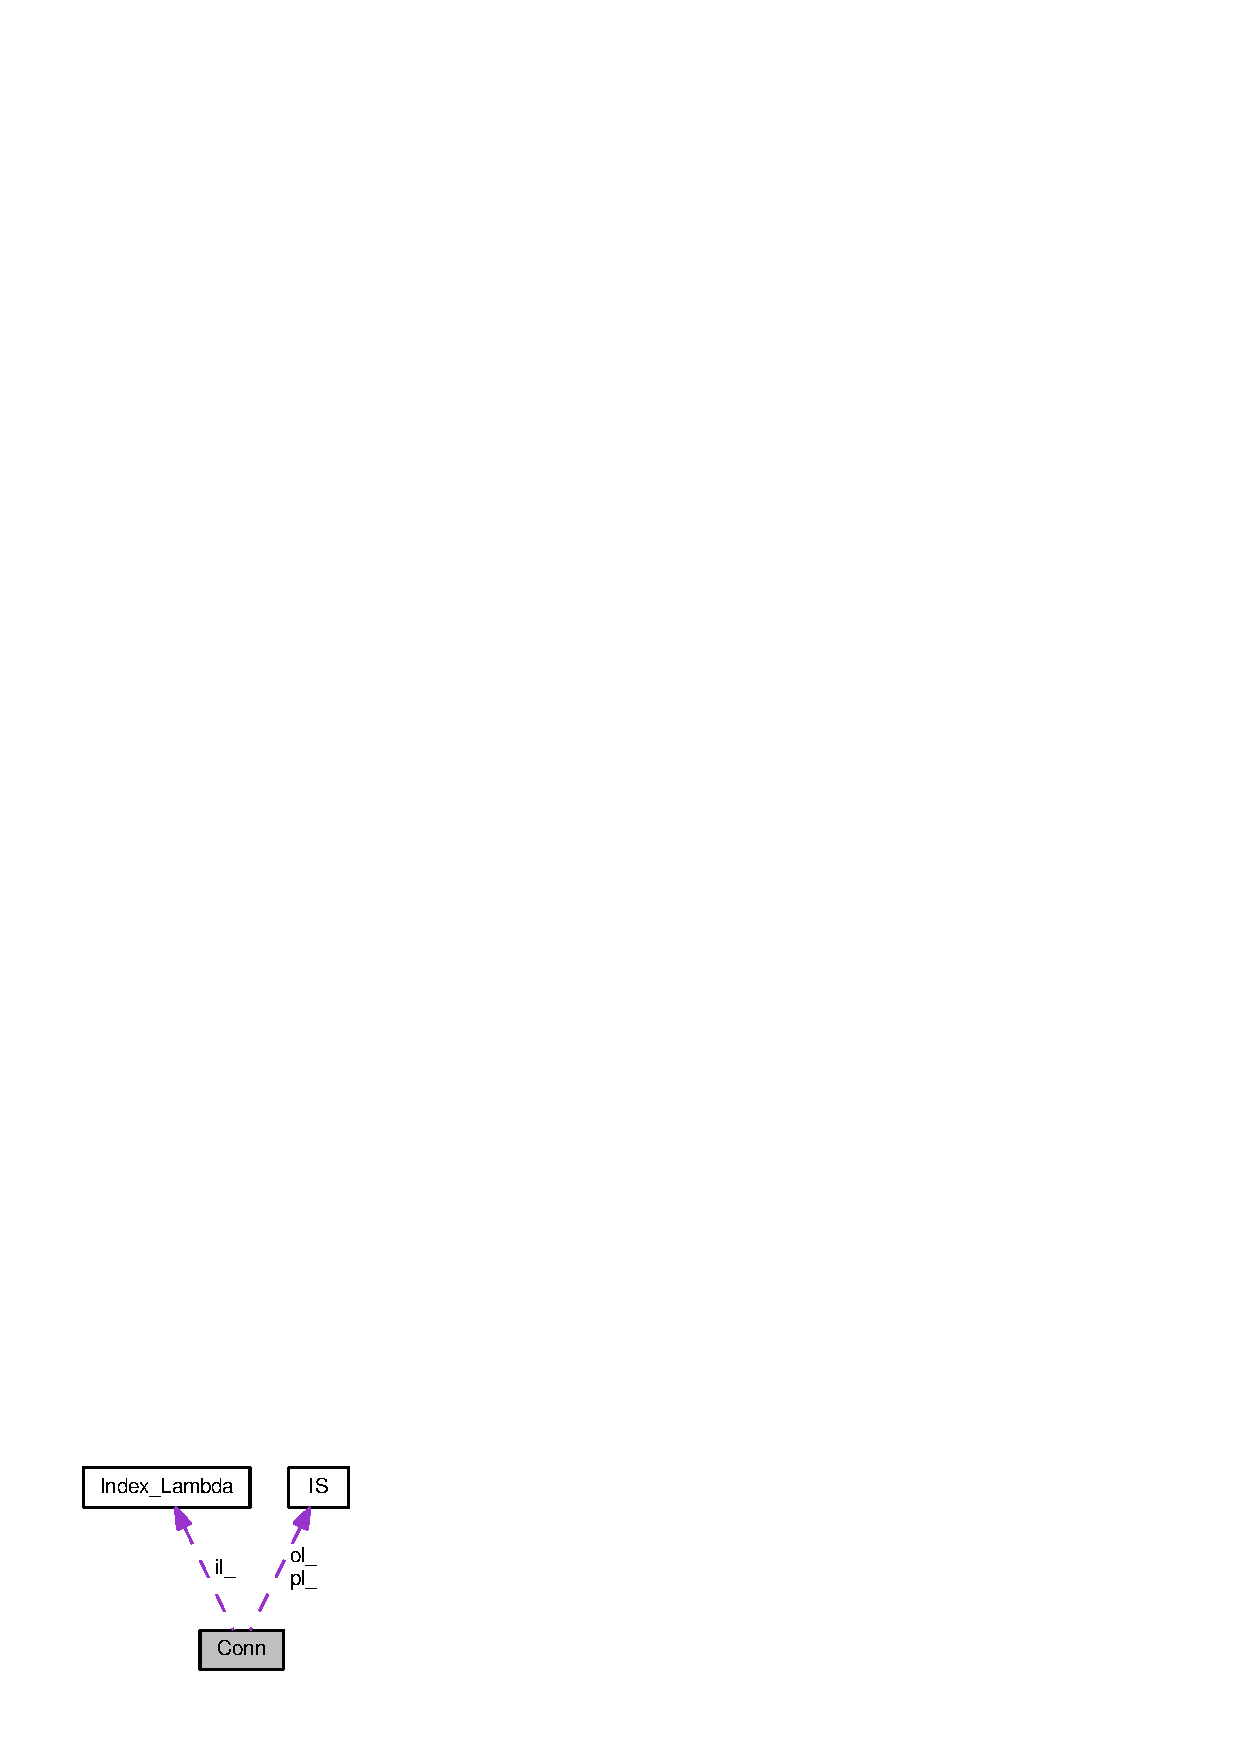
\includegraphics[width=172pt]{classConn__coll__graph}
\end{center}
\end{figure}
\subsection*{Public Member Functions}
\begin{DoxyCompactItemize}
\item 
\hypertarget{classConn_ab0ba4fbd67bc99991f2110c3ca80ca3d}{
{\bfseries Conn} (Face\_\-s face, void $\ast$conns)}
\label{classConn_ab0ba4fbd67bc99991f2110c3ca80ca3d}

\item 
\hypertarget{classConn_af3776731e374e856bb5eac3faea03ae3}{
void {\bfseries refresh} ()}
\label{classConn_af3776731e374e856bb5eac3faea03ae3}

\item 
\hypertarget{classConn_add96cc92a7575634f44220cb6e2e2421}{
void {\bfseries printinfo} ()}
\label{classConn_add96cc92a7575634f44220cb6e2e2421}

\item 
\hypertarget{classConn_ace36b6085ceadcfa9654b5950e7719c0}{
void {\bfseries send} (std::string name, array$<$ real, 1 $>$ v)}
\label{classConn_ace36b6085ceadcfa9654b5950e7719c0}

\item 
\hypertarget{classConn_a5f149a3217d7cf6227b48571638cadf8}{
array$<$ real, 1 $>$ {\bfseries recv} (std::string name)}
\label{classConn_a5f149a3217d7cf6227b48571638cadf8}

\end{DoxyCompactItemize}
\subsection*{Public Attributes}
\begin{DoxyCompactItemize}
\item 
\hypertarget{classConn_a61c9d519b93b91a14b4cc47a8cb8980b}{
\hyperlink{structIS}{IS} {\bfseries pl\_\-}}
\label{classConn_a61c9d519b93b91a14b4cc47a8cb8980b}

\item 
\hypertarget{classConn_a949773005bd6449b09e355e8f78dee47}{
\hyperlink{structIS}{IS} {\bfseries ol\_\-}}
\label{classConn_a949773005bd6449b09e355e8f78dee47}

\item 
\hypertarget{classConn_a8550bde616100c5f9cc23bc7ae267a18}{
int {\bfseries PG\_\-}}
\label{classConn_a8550bde616100c5f9cc23bc7ae267a18}

\item 
\hypertarget{classConn_a659caee9d9a125f24d7eb054ca2e5879}{
\hyperlink{structIndex__Lambda}{Index\_\-Lambda} {\bfseries il\_\-}}
\label{classConn_a659caee9d9a125f24d7eb054ca2e5879}

\item 
\hypertarget{classConn_a893abc608e559f12c5368edbd6da7b54}{
Face\_\-s {\bfseries face\_\-}}
\label{classConn_a893abc608e559f12c5368edbd6da7b54}

\item 
\hypertarget{classConn_a7578b2f58e208173f45436d7261271a0}{
Conn\_\-s {\bfseries twin\_\-}}
\label{classConn_a7578b2f58e208173f45436d7261271a0}

\item 
\hypertarget{classConn_ac571dea0fa3d37ed022872da32ad6c33}{
void $\ast$ {\bfseries conns\_\-}}
\label{classConn_ac571dea0fa3d37ed022872da32ad6c33}

\item 
\hypertarget{classConn_aae3bc6691f2e065bf44e8f1a2cd4e31f}{
bool {\bfseries parallel\_\-}}
\label{classConn_aae3bc6691f2e065bf44e8f1a2cd4e31f}

\item 
\hypertarget{classConn_a425d7d5713a82acbfa9a69adcc0c1c25}{
std::map$<$ std::string, array$<$ real, 1 $>$ $>$ {\bfseries equs\_\-}}
\label{classConn_a425d7d5713a82acbfa9a69adcc0c1c25}

\end{DoxyCompactItemize}


The documentation for this class was generated from the following files:\begin{DoxyCompactItemize}
\item 
src/Diff2D/conn.hpp\item 
src/Diff2D/conn.cpp\end{DoxyCompactItemize}

\hypertarget{structEdgeError}{
\section{EdgeError Struct Reference}
\label{structEdgeError}\index{EdgeError@{EdgeError}}
}
\subsection*{Public Member Functions}
\begin{DoxyCompactItemize}
\item 
\hypertarget{structEdgeError_a92ca9588f65b2b4d17139ff80eb29ab3}{
{\bfseries EdgeError} (bool rev)}
\label{structEdgeError_a92ca9588f65b2b4d17139ff80eb29ab3}

\item 
\hypertarget{structEdgeError_a92ca9588f65b2b4d17139ff80eb29ab3}{
{\bfseries EdgeError} (bool rev)}
\label{structEdgeError_a92ca9588f65b2b4d17139ff80eb29ab3}

\end{DoxyCompactItemize}
\subsection*{Public Attributes}
\begin{DoxyCompactItemize}
\item 
\hypertarget{structEdgeError_a704a81b20878f5b534df310ea179ae02}{
bool {\bfseries rev\_\-}}
\label{structEdgeError_a704a81b20878f5b534df310ea179ae02}

\end{DoxyCompactItemize}


The documentation for this struct was generated from the following files:\begin{DoxyCompactItemize}
\item 
src/Diff2D/util.cpp\item 
src/Diff2D/util.hpp\end{DoxyCompactItemize}

\hypertarget{classEquation}{\section{Equation Class Reference}
\label{classEquation}\index{Equation@{Equation}}
}


Collaboration diagram for Equation\-:
\nopagebreak
\begin{figure}[H]
\begin{center}
\leavevmode
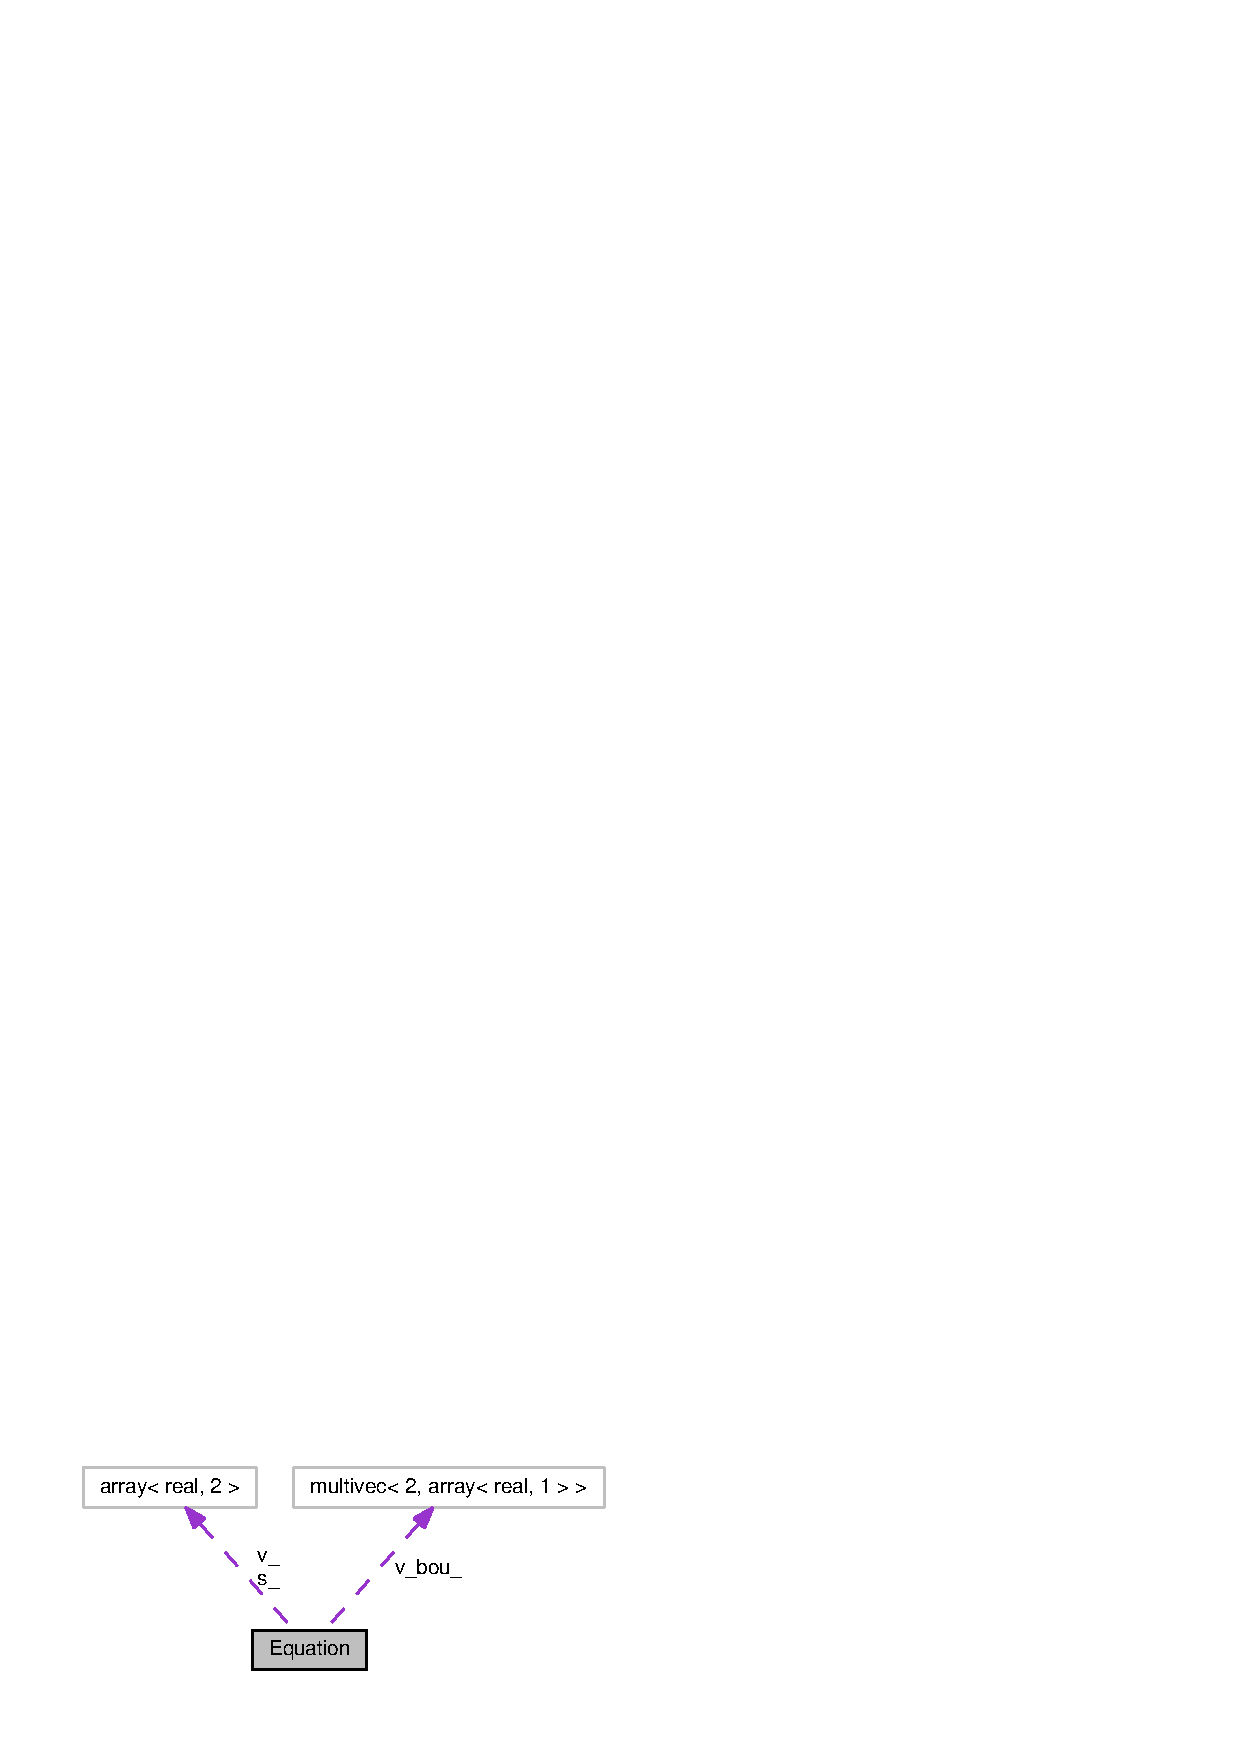
\includegraphics[width=274pt]{classEquation__coll__graph}
\end{center}
\end{figure}
\subsection*{Public Types}
\begin{DoxyCompactItemize}
\item 
enum \{ {\bfseries O\-N\-L\-Y\-\_\-\-P\-A\-R\-A\-L\-L\-E\-L\-\_\-\-F\-A\-C\-E\-S} =  1 $<$$<$ 0
 \}
\end{DoxyCompactItemize}
\subsection*{Public Member Functions}
\begin{DoxyCompactItemize}
\item 
\hypertarget{classEquation_aa828f4c9f7a849e9ae29f2c9491863d6}{{\bfseries Equation} (std\-::string name, Face\-\_\-s face, Equation\-\_\-\-Prob\-\_\-s equ\-\_\-prob)}\label{classEquation_aa828f4c9f7a849e9ae29f2c9491863d6}

\item 
\hypertarget{classEquation_acda03fc82a1a28ab32f127754bf37aea}{array$<$ real, 3 $>$ {\bfseries grad} ()}\label{classEquation_acda03fc82a1a28ab32f127754bf37aea}

\item 
\hypertarget{classEquation_ab67fb5e35d95e74756aed668b072c03f}{real {\bfseries grad\-\_\-mag} ()}\label{classEquation_ab67fb5e35d95e74756aed668b072c03f}

\item 
\hypertarget{classEquation_a629f1ff3c54e7fcfe597c20ab49c773b}{real {\bfseries min} ()}\label{classEquation_a629f1ff3c54e7fcfe597c20ab49c773b}

\item 
\hypertarget{classEquation_a1e95e7d54591e5dc5c68ccca547101c5}{real {\bfseries max} ()}\label{classEquation_a1e95e7d54591e5dc5c68ccca547101c5}

\item 
\hypertarget{classEquation_a3a22bc1a6dd067b6feaf6fc6281a5c1f}{real {\bfseries grad\-\_\-min} ()}\label{classEquation_a3a22bc1a6dd067b6feaf6fc6281a5c1f}

\item 
\hypertarget{classEquation_ae2b284533eda56200c9122846623eb45}{real {\bfseries grad\-\_\-max} ()}\label{classEquation_ae2b284533eda56200c9122846623eb45}

\item 
\hypertarget{classEquation_ae0198edcc6a9a44ed7d88d8279f91cee}{real {\bfseries mean} ()}\label{classEquation_ae0198edcc6a9a44ed7d88d8279f91cee}

\end{DoxyCompactItemize}
\subsection*{Public Attributes}
\begin{DoxyCompactItemize}
\item 
\hypertarget{classEquation_a2bbb65c98ebf1345231370e93b504037}{std\-::string {\bfseries name\-\_\-}}\label{classEquation_a2bbb65c98ebf1345231370e93b504037}

\item 
\hypertarget{classEquation_a9eeeceed0d8130fd30fb2e65f3b15f3f}{Face\-\_\-s {\bfseries face\-\_\-}}\label{classEquation_a9eeeceed0d8130fd30fb2e65f3b15f3f}

\item 
\hypertarget{classEquation_a1ece93bf1c58eb22001327da69ab73fc}{Equation\-\_\-\-Prob\-\_\-s {\bfseries equ\-\_\-prob\-\_\-}}\label{classEquation_a1ece93bf1c58eb22001327da69ab73fc}

\item 
\hypertarget{classEquation_ac7f793f3b1e3694b719d91d884460880}{array$<$ real, 2 $>$ {\bfseries s\-\_\-}}\label{classEquation_ac7f793f3b1e3694b719d91d884460880}

\item 
\hypertarget{classEquation_aa48c28c116aec278f7713a414dec6196}{array$<$ real, 2 $>$ {\bfseries v\-\_\-}}\label{classEquation_aa48c28c116aec278f7713a414dec6196}

\item 
\hypertarget{classEquation_a1820f1ab792e83981456fce5dda492b9}{unsigned int {\bfseries flag\-\_\-}}\label{classEquation_a1820f1ab792e83981456fce5dda492b9}

\item 
\hypertarget{classEquation_ab4039b291316d3a42c43330e868b4f50}{multivec$<$ 2, array$<$ real, 1 $>$ $>$ {\bfseries v\-\_\-bou\-\_\-}}\label{classEquation_ab4039b291316d3a42c43330e868b4f50}

\end{DoxyCompactItemize}


The documentation for this class was generated from the following files\-:\begin{DoxyCompactItemize}
\item 
src/\-Diff2\-D/equation.\-hpp\item 
src/\-Diff2\-D/equation.\-cpp\end{DoxyCompactItemize}

\hypertarget{classEquation__Prob}{
\section{Equation\_\-Prob Class Reference}
\label{classEquation__Prob}\index{Equation\_\-Prob@{Equation\_\-Prob}}
}
\subsection*{Public Member Functions}
\begin{DoxyCompactItemize}
\item 
\hypertarget{classEquation__Prob_a8eda60c6fe1e289ac5384cdf530cb47b}{
{\bfseries Equation\_\-Prob} (Prob\_\-s prob, std::string name, real k, real alpha, real alpha\_\-source)}
\label{classEquation__Prob_a8eda60c6fe1e289ac5384cdf530cb47b}

\end{DoxyCompactItemize}
\subsection*{Public Attributes}
\begin{DoxyCompactItemize}
\item 
\hypertarget{classEquation__Prob_a8761e4cfb7c9c934d1827a91625d7643}{
Prob\_\-s {\bfseries prob\_\-}}
\label{classEquation__Prob_a8761e4cfb7c9c934d1827a91625d7643}

\item 
\hypertarget{classEquation__Prob_af9c78d17a5b69f44175e95cef57c05d3}{
std::string {\bfseries name\_\-}}
\label{classEquation__Prob_af9c78d17a5b69f44175e95cef57c05d3}

\item 
\hypertarget{classEquation__Prob_add8db541a0ff4a402b95e2a70a3ad7a8}{
real {\bfseries k\_\-}}
\label{classEquation__Prob_add8db541a0ff4a402b95e2a70a3ad7a8}

\item 
\hypertarget{classEquation__Prob_ab8c2b9f46d6d9393c6556d0e734aae61}{
real {\bfseries alpha\_\-}}
\label{classEquation__Prob_ab8c2b9f46d6d9393c6556d0e734aae61}

\item 
\hypertarget{classEquation__Prob_aeb3f0d6aa0ffbbd16bc0866f177ec13e}{
real {\bfseries alpha\_\-source\_\-}}
\label{classEquation__Prob_aeb3f0d6aa0ffbbd16bc0866f177ec13e}

\end{DoxyCompactItemize}


The documentation for this class was generated from the following files:\begin{DoxyCompactItemize}
\item 
src/Diff2D/equation.hpp\item 
src/Diff2D/equation.cpp\end{DoxyCompactItemize}

\hypertarget{classFace}{\section{Face Class Reference}
\label{classFace}\index{Face@{Face}}
}


Inheritance diagram for Face\-:\nopagebreak
\begin{figure}[H]
\begin{center}
\leavevmode
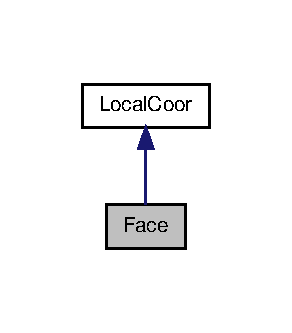
\includegraphics[width=140pt]{classFace__inherit__graph}
\end{center}
\end{figure}


Collaboration diagram for Face\-:\nopagebreak
\begin{figure}[H]
\begin{center}
\leavevmode
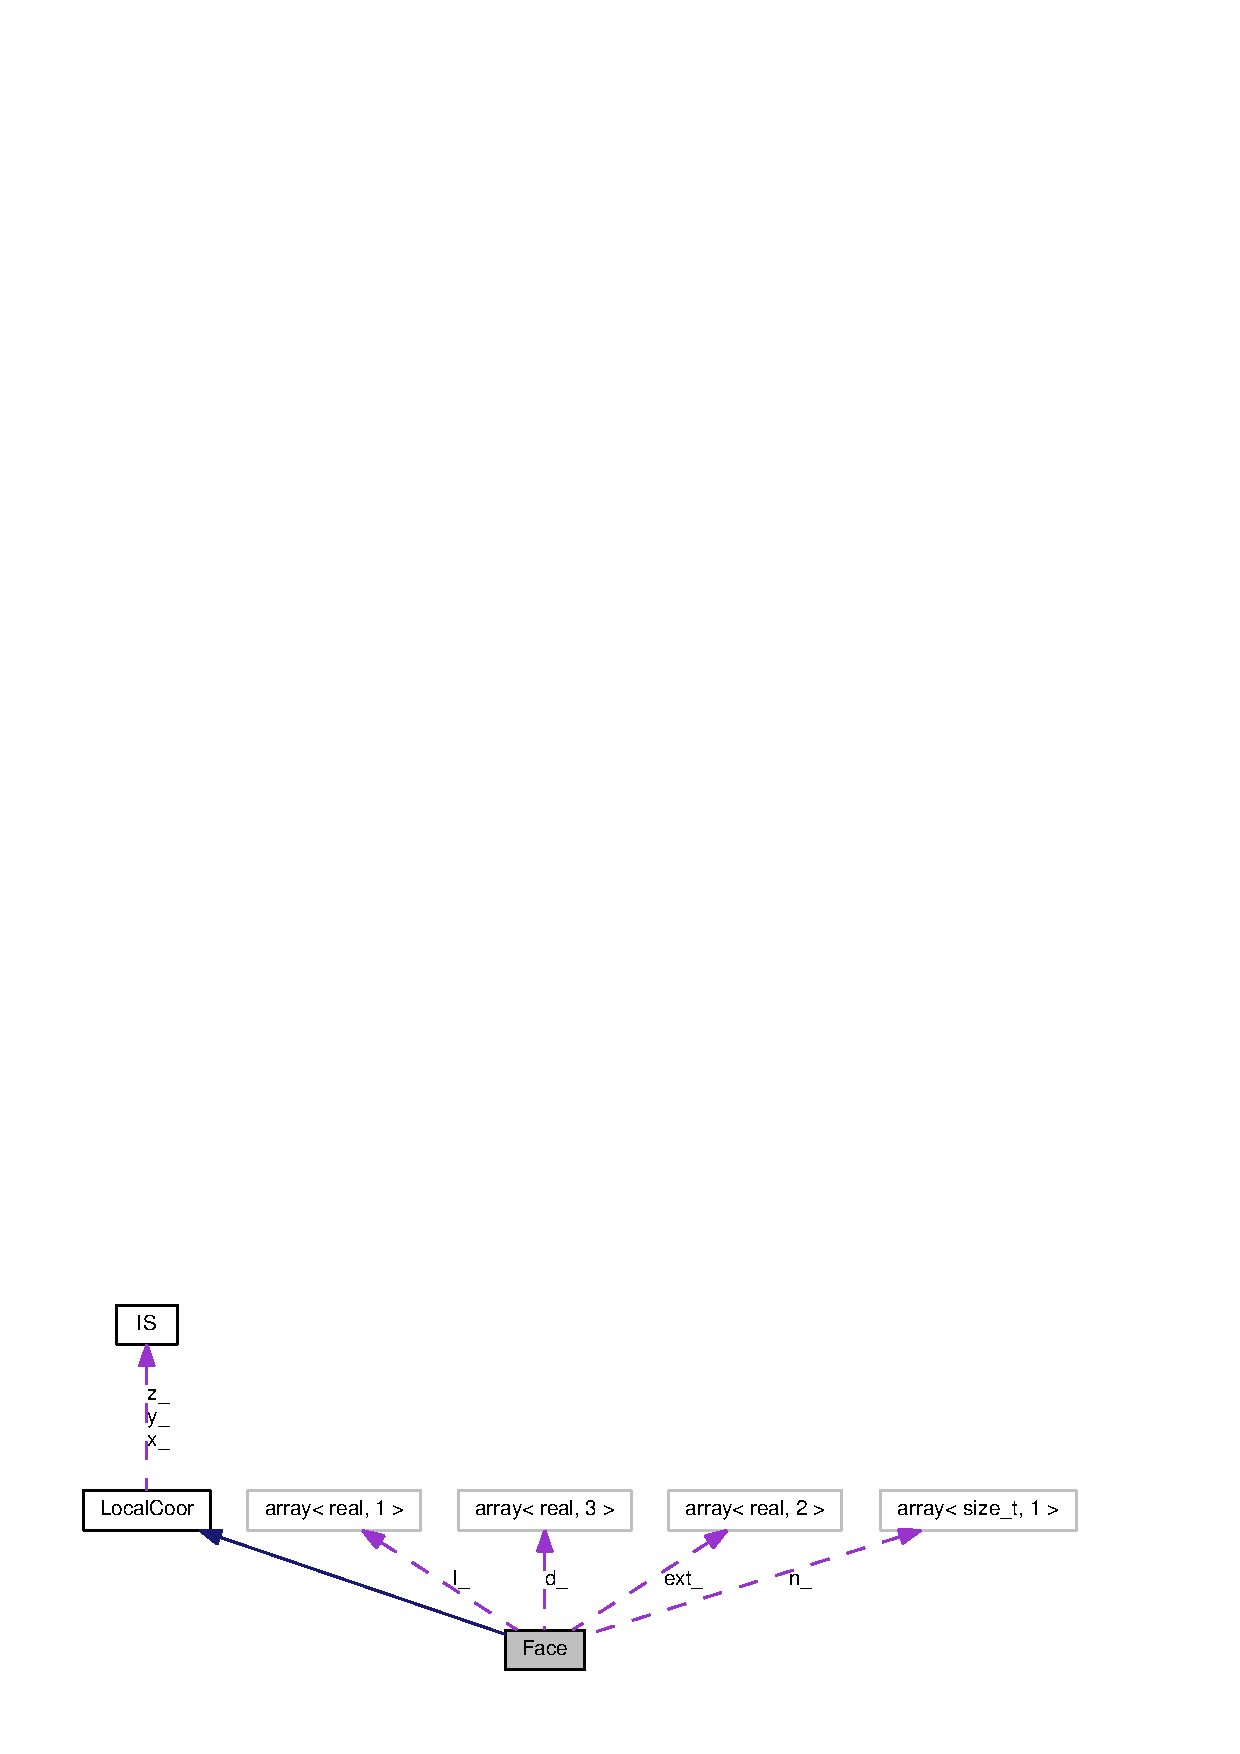
\includegraphics[width=350pt]{classFace__coll__graph}
\end{center}
\end{figure}
\subsection*{Public Member Functions}
\begin{DoxyCompactItemize}
\item 
\hypertarget{classFace_a3b8f88dfdae278eb7ac120e3a09ae333}{{\bfseries Face} (Patch\-\_\-s patch, int normal, array$<$ real, 2 $>$ const \&ext, real pos\-\_\-z, array$<$ int, 1 $>$ n)}\label{classFace_a3b8f88dfdae278eb7ac120e3a09ae333}

\item 
\hypertarget{classFace_a23e698d2341c3634212729c78bba154f}{void {\bfseries create\-\_\-equ} (std\-::string name, Equation\-\_\-\-Prob\-\_\-s equ\-\_\-prob)}\label{classFace_a23e698d2341c3634212729c78bba154f}

\item 
\hypertarget{classFace_a7ebc4163752a05d82e184a3a4c8671b3}{int {\bfseries get\-\_\-loc\-\_\-pos\-\_\-par\-\_\-index} (Face\-\_\-s nbr)}\label{classFace_a7ebc4163752a05d82e184a3a4c8671b3}

\item 
\hypertarget{classFace_aed5980668f26bc29338dfa11b32919f5}{real {\bfseries x} (int i)}\label{classFace_aed5980668f26bc29338dfa11b32919f5}

\item 
\hypertarget{classFace_a9a4d892bf5e8782c898e15aa5a989806}{real {\bfseries y} (int j)}\label{classFace_a9a4d892bf5e8782c898e15aa5a989806}

\item 
\hypertarget{classFace_a2d20ebd0d99063967bb26657abebbcbe}{real {\bfseries area} ()}\label{classFace_a2d20ebd0d99063967bb26657abebbcbe}

\item 
\hypertarget{classFace_a06eb55371bc742e523a9eb94a573209d}{int {\bfseries nbr\-\_\-to\-\_\-loc} (Face\-\_\-s nbr)}\label{classFace_a06eb55371bc742e523a9eb94a573209d}

\item 
\hypertarget{classFace_a60baec409a104a88e6622efa2f80122c}{Conn\-\_\-s {\bfseries loc\-\_\-to\-\_\-conn} (int V)}\label{classFace_a60baec409a104a88e6622efa2f80122c}

\item 
\hypertarget{classFace_a9a5eb93863dc767848261afa813ca039}{\hyperlink{structIndex__Lambda}{Index\-\_\-\-Lambda} {\bfseries index\-\_\-lambda} (Face\-\_\-s nbr)}\label{classFace_a9a5eb93863dc767848261afa813ca039}

\item 
\hypertarget{classFace_afdbbc9947c0d7cd84b427bd7b503b15b}{void {\bfseries send\-\_\-array} (Equation\-\_\-s equ, Conn\-\_\-s conn)}\label{classFace_afdbbc9947c0d7cd84b427bd7b503b15b}

\item 
\hypertarget{classFace_a57bdfcf1ebf5e208b611f98b7ddeca00}{void {\bfseries recv\-\_\-array} (Equation\-\_\-s equ, Conn\-\_\-s conn)}\label{classFace_a57bdfcf1ebf5e208b611f98b7ddeca00}

\item 
\hypertarget{classFace_aa827a7d26d1b90507bb4252830b3ecf5}{\hyperlink{structTerm}{Term} {\bfseries term} (Equation\-\_\-s equ, std\-::vector$<$ int $>$ ind, int v, int sv, real To)}\label{classFace_aa827a7d26d1b90507bb4252830b3ecf5}

\item 
\hypertarget{classFace_aba0d776b0f0e7cceee8729825347b5cc}{void {\bfseries step\-\_\-pre\-\_\-cell} (Equation\-\_\-s equ, std\-::vector$<$ int $>$ ind, int V)}\label{classFace_aba0d776b0f0e7cceee8729825347b5cc}

\item 
\hypertarget{classFace_a2bafbcce9f57fd3bdefd9f23a62c853d}{void {\bfseries step\-\_\-pre\-\_\-cell\-\_\-open\-\_\-bou} (Equation\-\_\-s equ, std\-::vector$<$ int $>$ ind, int V)}\label{classFace_a2bafbcce9f57fd3bdefd9f23a62c853d}

\item 
\hypertarget{classFace_a8af2298846b8a666332f00de91796844}{void {\bfseries step\-\_\-pre} (Equation\-\_\-s equ)}\label{classFace_a8af2298846b8a666332f00de91796844}

\item 
\hypertarget{classFace_a62a7d504c1e99dfc928b7e27b544893b}{real {\bfseries step} (std\-::string equ\-\_\-name)}\label{classFace_a62a7d504c1e99dfc928b7e27b544893b}

\item 
\hypertarget{classFace_a781b3843f33507116afa741579317e83}{void {\bfseries send} (std\-::string equ\-\_\-name)}\label{classFace_a781b3843f33507116afa741579317e83}

\item 
\hypertarget{classFace_a4c67c45fa975e6fb3bc3d4ee0fa6a25f}{void {\bfseries recv} (std\-::string equ\-\_\-name)}\label{classFace_a4c67c45fa975e6fb3bc3d4ee0fa6a25f}

\item 
\hypertarget{classFace_a18aba75abf718dd35c17153220ad929b}{grid\-\_\-tup {\bfseries grid} (std\-::string equ\-\_\-name)}\label{classFace_a18aba75abf718dd35c17153220ad929b}

\end{DoxyCompactItemize}
\subsection*{Public Attributes}
\begin{DoxyCompactItemize}
\item 
\hypertarget{classFace_a2e53c055a4d8492b42995db563e1fc7a}{Patch\-\_\-s {\bfseries patch\-\_\-}}\label{classFace_a2e53c055a4d8492b42995db563e1fc7a}

\item 
\hypertarget{classFace_a0922668c4175d0274024a5869b310a63}{array$<$ real, 2 $>$ {\bfseries ext\-\_\-}}\label{classFace_a0922668c4175d0274024a5869b310a63}

\item 
\hypertarget{classFace_a639f6d684b3a55d69528b5b6f5976937}{real {\bfseries pos\-\_\-z\-\_\-}}\label{classFace_a639f6d684b3a55d69528b5b6f5976937}

\item 
\hypertarget{classFace_ab9b865c72ed43ab63dd5747639bd13f1}{array$<$ int, 1 $>$ {\bfseries n\-\_\-}}\label{classFace_ab9b865c72ed43ab63dd5747639bd13f1}

\item 
\hypertarget{classFace_a7d41239f934e8819874b5fb515d43380}{array$<$ real, 3 $>$ {\bfseries d\-\_\-}}\label{classFace_a7d41239f934e8819874b5fb515d43380}

\item 
\hypertarget{classFace_a75033fb2521fcb2c613782f831f42bb3}{array$<$ real, 1 $>$ {\bfseries l\-\_\-}}\label{classFace_a75033fb2521fcb2c613782f831f42bb3}

\item 
\hypertarget{classFace_a46b37a1eaba00ad44cf46b6da1391b30}{std\-::map$<$ std\-::string, Equation\-\_\-s $>$ {\bfseries equs\-\_\-}}\label{classFace_a46b37a1eaba00ad44cf46b6da1391b30}

\item 
\hypertarget{classFace_ac831a8581fa641c54f4adb6e6b3dfe71}{std\-::vector$<$ std\-::vector\\*
$<$ Conn\-\_\-s $>$ $>$ {\bfseries conns\-\_\-}}\label{classFace_ac831a8581fa641c54f4adb6e6b3dfe71}

\item 
\hypertarget{classFace_a982045b07b690ea86fc8faa77a1cc534}{std\-::map$<$ std\-::string, array\\*
$<$ real, 1 $>$\mbox{[}2\mbox{]}\mbox{[}2\mbox{]}$>$ {\bfseries v\-\_\-bou\-\_\-}}\label{classFace_a982045b07b690ea86fc8faa77a1cc534}

\end{DoxyCompactItemize}


The documentation for this class was generated from the following files\-:\begin{DoxyCompactItemize}
\item 
src/\-Diff2\-D/face.\-hpp\item 
src/\-Diff2\-D/face.\-cpp\end{DoxyCompactItemize}

\hypertarget{structIndex__Lambda}{
\section{Index\_\-Lambda Struct Reference}
\label{structIndex__Lambda}\index{Index\_\-Lambda@{Index\_\-Lambda}}
}
\subsection*{Public Member Functions}
\begin{DoxyCompactItemize}
\item 
\hypertarget{structIndex__Lambda_af8225252f38290763a8aae14a0660a02}{
int {\bfseries operator()} (int i, int p)}
\label{structIndex__Lambda_af8225252f38290763a8aae14a0660a02}

\end{DoxyCompactItemize}
\subsection*{Public Attributes}
\begin{DoxyCompactItemize}
\item 
\hypertarget{structIndex__Lambda_acdf68b7c6f870f4eeb4ee9d8183e0c73}{
int {\bfseries a} \mbox{[}2\mbox{]}}
\label{structIndex__Lambda_acdf68b7c6f870f4eeb4ee9d8183e0c73}

\item 
\hypertarget{structIndex__Lambda_aaa095d0d1b30bc698d5a816ff0199951}{
int {\bfseries b} \mbox{[}2\mbox{]}}
\label{structIndex__Lambda_aaa095d0d1b30bc698d5a816ff0199951}

\item 
\hypertarget{structIndex__Lambda_a34e9306034a5059d37f4ab53d79ea5c7}{
real {\bfseries d}}
\label{structIndex__Lambda_a34e9306034a5059d37f4ab53d79ea5c7}

\end{DoxyCompactItemize}


The documentation for this struct was generated from the following file:\begin{DoxyCompactItemize}
\item 
src/Diff2D/index\_\-lambda.hpp\end{DoxyCompactItemize}

\hypertarget{structInitializer__list}{\section{Initializer\-\_\-list$<$ D, U $>$ Struct Template Reference}
\label{structInitializer__list}\index{Initializer\-\_\-list$<$ D, U $>$@{Initializer\-\_\-list$<$ D, U $>$}}
}
\subsection*{Public Types}
\begin{DoxyCompactItemize}
\item 
\hypertarget{structInitializer__list_ae28944fda227672ee3e7bac608a7b30a}{typedef std\-::initializer\-\_\-list\\*
$<$ typename \hyperlink{structInitializer__list}{Initializer\-\_\-list}$<$ D-\/1, \\*
U $>$\-::list\-\_\-type $>$ {\bfseries list\-\_\-type}}\label{structInitializer__list_ae28944fda227672ee3e7bac608a7b30a}

\end{DoxyCompactItemize}


The documentation for this struct was generated from the following file\-:\begin{DoxyCompactItemize}
\item 
src/\-Diff2\-D/array.\-hpp\end{DoxyCompactItemize}

\hypertarget{structInitializer__list_3_011_00_01U_01_4}{\section{Initializer\-\_\-list$<$ 1, U $>$ Struct Template Reference}
\label{structInitializer__list_3_011_00_01U_01_4}\index{Initializer\-\_\-list$<$ 1, U $>$@{Initializer\-\_\-list$<$ 1, U $>$}}
}
\subsection*{Public Types}
\begin{DoxyCompactItemize}
\item 
\hypertarget{structInitializer__list_3_011_00_01U_01_4_a84155c0e2c82ce1298dfa8ae00c670c6}{typedef std\-::initializer\-\_\-list$<$ U $>$ {\bfseries list\-\_\-type}}\label{structInitializer__list_3_011_00_01U_01_4_a84155c0e2c82ce1298dfa8ae00c670c6}

\end{DoxyCompactItemize}


The documentation for this struct was generated from the following file\-:\begin{DoxyCompactItemize}
\item 
src/\-Diff2\-D/array.\-hpp\end{DoxyCompactItemize}

\hypertarget{structIS}{
\section{IS Struct Reference}
\label{structIS}\index{IS@{IS}}
}
\subsection*{Public Member Functions}
\begin{DoxyCompactItemize}
\item 
\hypertarget{structIS_aec66c50fd699031a1f617117c67eda11}{
\hyperlink{structIS}{IS} \& {\bfseries operator=} (\hyperlink{structIS}{IS} const \&is)}
\label{structIS_aec66c50fd699031a1f617117c67eda11}

\item 
\hypertarget{structIS_a2cb6d148c70406c11b9508be2cfddd7e}{
{\bfseries IS} (int ni, int ns)}
\label{structIS_a2cb6d148c70406c11b9508be2cfddd7e}

\item 
\hypertarget{structIS_a53883df04399eab305d240898e889271}{
{\bfseries IS} (int v)}
\label{structIS_a53883df04399eab305d240898e889271}

\item 
\hypertarget{structIS_ad474289c5f0f5f5b231cd2067547cc0f}{
int {\bfseries v} ()}
\label{structIS_ad474289c5f0f5f5b231cd2067547cc0f}

\end{DoxyCompactItemize}
\subsection*{Public Attributes}
\begin{DoxyCompactItemize}
\item 
\hypertarget{structIS_ac0a890989ec0d04b8db157583b154c17}{
int {\bfseries i}}
\label{structIS_ac0a890989ec0d04b8db157583b154c17}

\item 
\hypertarget{structIS_a3a4dc37a5dc69fa81e33c5e7115dca71}{
int {\bfseries s}}
\label{structIS_a3a4dc37a5dc69fa81e33c5e7115dca71}

\end{DoxyCompactItemize}


The documentation for this struct was generated from the following file:\begin{DoxyCompactItemize}
\item 
src/Diff2D/unit\_\-vec.hpp\end{DoxyCompactItemize}

\hypertarget{classLocalCoor}{\section{Local\-Coor Class Reference}
\label{classLocalCoor}\index{Local\-Coor@{Local\-Coor}}
}


Inheritance diagram for Local\-Coor\-:\nopagebreak
\begin{figure}[H]
\begin{center}
\leavevmode
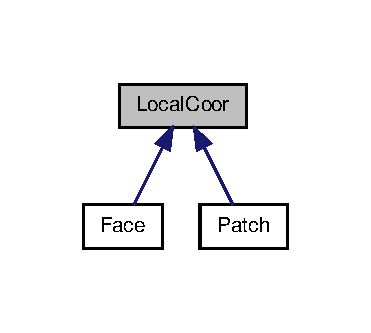
\includegraphics[width=178pt]{classLocalCoor__inherit__graph}
\end{center}
\end{figure}


Collaboration diagram for Local\-Coor\-:\nopagebreak
\begin{figure}[H]
\begin{center}
\leavevmode
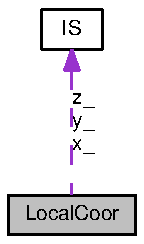
\includegraphics[width=140pt]{classLocalCoor__coll__graph}
\end{center}
\end{figure}
\subsection*{Public Member Functions}
\begin{DoxyCompactItemize}
\item 
\hypertarget{classLocalCoor_a00f6c0c9e48e46f15e1aaf36331fedeb}{{\bfseries Local\-Coor} (int Z)}\label{classLocalCoor_a00f6c0c9e48e46f15e1aaf36331fedeb}

\item 
\hypertarget{classLocalCoor_ab96f489ba970f19b22e75f94bbec99c1}{int {\bfseries glo\-\_\-to\-\_\-loc} (int G)}\label{classLocalCoor_ab96f489ba970f19b22e75f94bbec99c1}

\item 
\hypertarget{classLocalCoor_ab5da8e4b3f6c32fbf6636aaa47e04adc}{int {\bfseries loc\-\_\-to\-\_\-glo} (int L)}\label{classLocalCoor_ab5da8e4b3f6c32fbf6636aaa47e04adc}

\end{DoxyCompactItemize}
\subsection*{Public Attributes}
\begin{DoxyCompactItemize}
\item 
\hypertarget{classLocalCoor_a7d72e3489aaf1b6579f7a3e0f5b30e26}{int {\bfseries X\-\_\-}}\label{classLocalCoor_a7d72e3489aaf1b6579f7a3e0f5b30e26}

\item 
\hypertarget{classLocalCoor_a5ff6668d5d6898582ddfdc5eadce58ff}{int {\bfseries Y\-\_\-}}\label{classLocalCoor_a5ff6668d5d6898582ddfdc5eadce58ff}

\item 
\hypertarget{classLocalCoor_acd97c2eb7e3b994dbc58ae98ab785280}{int {\bfseries Z\-\_\-}}\label{classLocalCoor_acd97c2eb7e3b994dbc58ae98ab785280}

\item 
\hypertarget{classLocalCoor_a2c0e974fc45c597f893b20a0c2f6869c}{\hyperlink{structIS}{I\-S} {\bfseries x\-\_\-}}\label{classLocalCoor_a2c0e974fc45c597f893b20a0c2f6869c}

\item 
\hypertarget{classLocalCoor_a58678d9cfb17db349a9d7fd70a2d5150}{\hyperlink{structIS}{I\-S} {\bfseries y\-\_\-}}\label{classLocalCoor_a58678d9cfb17db349a9d7fd70a2d5150}

\item 
\hypertarget{classLocalCoor_acdd6d24c450a43fd755f2e43d16d9991}{\hyperlink{structIS}{I\-S} {\bfseries z\-\_\-}}\label{classLocalCoor_acdd6d24c450a43fd755f2e43d16d9991}

\end{DoxyCompactItemize}


The documentation for this class was generated from the following file\-:\begin{DoxyCompactItemize}
\item 
src/\-Diff2\-D/unit\-\_\-vec.\-hpp\end{DoxyCompactItemize}

\hypertarget{structNoIntersectError}{
\section{NoIntersectError Struct Reference}
\label{structNoIntersectError}\index{NoIntersectError@{NoIntersectError}}
}


The documentation for this struct was generated from the following file:\begin{DoxyCompactItemize}
\item 
src/Diff2D/util.cpp\end{DoxyCompactItemize}

\hypertarget{classPatch}{\section{Patch Class Reference}
\label{classPatch}\index{Patch@{Patch}}
}


Inheritance diagram for Patch\-:\nopagebreak
\begin{figure}[H]
\begin{center}
\leavevmode
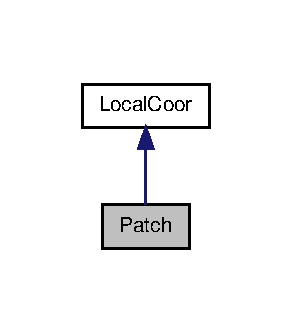
\includegraphics[width=140pt]{classPatch__inherit__graph}
\end{center}
\end{figure}


Collaboration diagram for Patch\-:\nopagebreak
\begin{figure}[H]
\begin{center}
\leavevmode
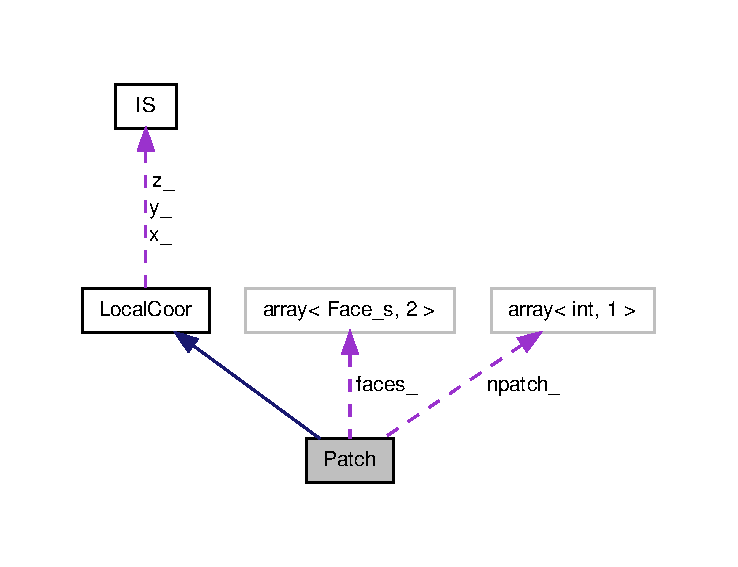
\includegraphics[width=350pt]{classPatch__coll__graph}
\end{center}
\end{figure}
\subsection*{Public Member Functions}
\begin{DoxyCompactItemize}
\item 
\hypertarget{classPatch_a7adac62309652817919b4e508782566d}{{\bfseries Patch} (Patch\-\_\-\-Group\-\_\-s group, std\-::string name, int normal, std\-::vector$<$ std\-::vector$<$ int $>$ $>$ indices, std\-::vector$<$ array$<$ real, 1 $>$ $>$ x, std\-::vector$<$ array$<$ int, 1 $>$ $>$ nx, v\-\_\-bou\-\_\-type v\-\_\-bou)}\label{classPatch_a7adac62309652817919b4e508782566d}

\item 
\hypertarget{classPatch_ac8352cc930b37975da9627262540cebd}{void {\bfseries create\-\_\-equ} (std\-::string name, real v0, std\-::vector$<$ array$<$ real, 1 $>$ $>$ v\-\_\-bou, real k, real al)}\label{classPatch_ac8352cc930b37975da9627262540cebd}

\item 
\hypertarget{classPatch_af0311eccfd4f4fd356785f7b23dc8fa2}{void {\bfseries set\-\_\-v\-\_\-bou} (std\-::string equ\-\_\-name, std\-::vector$<$ array$<$ real, 1 $>$ $>$ v\-\_\-bou)}\label{classPatch_af0311eccfd4f4fd356785f7b23dc8fa2}

\item 
\hypertarget{classPatch_aa0a6036ed90bf4a98cc498f925fb530d}{real {\bfseries max} (std\-::string equ\-\_\-name)}\label{classPatch_aa0a6036ed90bf4a98cc498f925fb530d}

\item 
\hypertarget{classPatch_ae57b4223cce6c1ed9dbaaa5080a2501a}{void {\bfseries grid\-\_\-nbrs} ()}\label{classPatch_ae57b4223cce6c1ed9dbaaa5080a2501a}

\end{DoxyCompactItemize}
\subsection*{Public Attributes}
\begin{DoxyCompactItemize}
\item 
\hypertarget{classPatch_a93fff2891647c4109c16cb4ec2079545}{Patch\-\_\-\-Group\-\_\-w {\bfseries group\-\_\-}}\label{classPatch_a93fff2891647c4109c16cb4ec2079545}

\item 
\hypertarget{classPatch_a133d268d88897aef8b20ca7da98b9cdb}{std\-::string {\bfseries name\-\_\-}}\label{classPatch_a133d268d88897aef8b20ca7da98b9cdb}

\item 
\hypertarget{classPatch_a9cf37e5da9a803692c4ad575ec3ffbb1}{std\-::vector$<$ std\-::vector$<$ int $>$ $>$ {\bfseries indices\-\_\-}}\label{classPatch_a9cf37e5da9a803692c4ad575ec3ffbb1}

\item 
\hypertarget{classPatch_a41ac7ad621e3c8c93014e96050985990}{array$<$ int, 1 $>$ {\bfseries npatch\-\_\-}}\label{classPatch_a41ac7ad621e3c8c93014e96050985990}

\item 
\hypertarget{classPatch_a6d0bbabb9b7b1928bda12255b312fedd}{array$<$ Face\-\_\-s, 2 $>$ {\bfseries faces\-\_\-}}\label{classPatch_a6d0bbabb9b7b1928bda12255b312fedd}

\end{DoxyCompactItemize}


The documentation for this class was generated from the following files\-:\begin{DoxyCompactItemize}
\item 
src/\-Diff2\-D/patch.\-hpp\item 
src/\-Diff2\-D/patch.\-cpp\end{DoxyCompactItemize}

\hypertarget{classPatch__Group}{\section{Patch\-\_\-\-Group Class Reference}
\label{classPatch__Group}\index{Patch\-\_\-\-Group@{Patch\-\_\-\-Group}}
}
\subsection*{Public Member Functions}
\begin{DoxyCompactItemize}
\item 
\hypertarget{classPatch__Group_a7585b36431136e14c2d17e84388969be}{{\bfseries Patch\-\_\-\-Group} (Prob\-\_\-s prob, std\-::string name, std\-::map$<$ std\-::string, real $>$ v\-\_\-0, std\-::map$<$ std\-::string, real $>$ S)}\label{classPatch__Group_a7585b36431136e14c2d17e84388969be}

\item 
\hypertarget{classPatch__Group_a77ed7a1c169f6131ba85329bfa2b2592}{Patch\-\_\-s {\bfseries create\-\_\-patch} (std\-::string name, int normal, std\-::vector$<$ std\-::vector$<$ int $>$ $>$ indices, v\-\_\-bou\-\_\-type v\-\_\-bou)}\label{classPatch__Group_a77ed7a1c169f6131ba85329bfa2b2592}

\item 
\hypertarget{classPatch__Group_ada9f56e3be9279ff5d555f2192cfc45b}{real {\bfseries reset\-\_\-s} (std\-::string equ\-\_\-name)}\label{classPatch__Group_ada9f56e3be9279ff5d555f2192cfc45b}

\item 
\hypertarget{classPatch__Group_a326628f83583bb2194f8c82548e9b6b3}{std\-::vector$<$ Face\-\_\-s $>$ {\bfseries faces} ()}\label{classPatch__Group_a326628f83583bb2194f8c82548e9b6b3}

\item 
\hypertarget{classPatch__Group_a3de7d3df9923795d4cbfa4d908e53598}{void {\bfseries write} (std\-::string equ\-\_\-name, std\-::ofstream \&ofs)}\label{classPatch__Group_a3de7d3df9923795d4cbfa4d908e53598}

\end{DoxyCompactItemize}
\subsection*{Public Attributes}
\begin{DoxyCompactItemize}
\item 
\hypertarget{classPatch__Group_a637b27a0562076f78bf9b0698ac3609e}{std\-::vector$<$ Patch\-\_\-s $>$ {\bfseries patches\-\_\-}}\label{classPatch__Group_a637b27a0562076f78bf9b0698ac3609e}

\item 
\hypertarget{classPatch__Group_ac8d91a179d394f1d3d355d82ceb2dd2e}{Prob\-\_\-w {\bfseries prob\-\_\-}}\label{classPatch__Group_ac8d91a179d394f1d3d355d82ceb2dd2e}

\item 
\hypertarget{classPatch__Group_ac28afa5068ea65b91ce4d708f63c5a3a}{std\-::string {\bfseries name\-\_\-}}\label{classPatch__Group_ac28afa5068ea65b91ce4d708f63c5a3a}

\item 
\hypertarget{classPatch__Group_ae080e43ddd30ced473794b12a1cb3ccf}{std\-::map$<$ std\-::string, real $>$ {\bfseries v\-\_\-0\-\_\-}}\label{classPatch__Group_ae080e43ddd30ced473794b12a1cb3ccf}

\item 
\hypertarget{classPatch__Group_aaad946bd88382b1e2e30cd1278632ace}{std\-::map$<$ std\-::string, real $>$ {\bfseries S\-\_\-}}\label{classPatch__Group_aaad946bd88382b1e2e30cd1278632ace}

\end{DoxyCompactItemize}


The documentation for this class was generated from the following files\-:\begin{DoxyCompactItemize}
\item 
src/\-Diff2\-D/patch\-\_\-group.\-hpp\item 
src/\-Diff2\-D/patch\-\_\-group.\-cpp\end{DoxyCompactItemize}

\hypertarget{classProb}{
\section{Prob Class Reference}
\label{classProb}\index{Prob@{Prob}}
}


Problem  


{\ttfamily \#include $<$prob.hpp$>$}\subsection*{Public Member Functions}
\begin{DoxyCompactItemize}
\item 
\hypertarget{classProb_a4d146873812b11594835eeb221057ce3}{
{\bfseries Prob} (std::string name, coor\_\-type x, cell\_\-count\_\-type nx, int it\_\-max\_\-1, int it\_\-max\_\-2)}
\label{classProb_a4d146873812b11594835eeb221057ce3}

\item 
\hypertarget{classProb_a9e42af858cc616a84ffa860ed30703cc}{
Equation\_\-Prob\_\-s {\bfseries create\_\-equation} (std::string name, real k, real alpha, real alpha\_\-source)}
\label{classProb_a9e42af858cc616a84ffa860ed30703cc}

\item 
\hypertarget{classProb_a3cc8bff1793014e79c9f543c6b06db37}{
Patch\_\-Group\_\-s {\bfseries create\_\-patch\_\-group} (std::string name, std::map$<$ std::string, real $>$ v\_\-0, std::map$<$ std::string, real $>$ S)}
\label{classProb_a3cc8bff1793014e79c9f543c6b06db37}

\item 
\hypertarget{classProb_a70dca1f3332e57f72b834ba91d52ca31}{
real {\bfseries temp\_\-max} (std::string equ\_\-name)}
\label{classProb_a70dca1f3332e57f72b834ba91d52ca31}

\item 
\hypertarget{classProb_ac1bce1f293f1ec1c251730db1a1d0313}{
real {\bfseries temp\_\-min} (std::string equ\_\-name)}
\label{classProb_ac1bce1f293f1ec1c251730db1a1d0313}

\item 
\hypertarget{classProb_a9fff19c6e6676c72153dc0ed32b1e6a9}{
real {\bfseries grad\_\-max} (std::string equ\_\-name)}
\label{classProb_a9fff19c6e6676c72153dc0ed32b1e6a9}

\item 
\hypertarget{classProb_a6dc764bdb12b430c1a28d73925f6c6d8}{
real {\bfseries grad\_\-min} (std::string equ\_\-name)}
\label{classProb_a6dc764bdb12b430c1a28d73925f6c6d8}

\item 
\hypertarget{classProb_aa5c8f3a5c0e9a15e054ca37d150a8921}{
void {\bfseries value\_\-add} (std::string equ\_\-name, real v)}
\label{classProb_aa5c8f3a5c0e9a15e054ca37d150a8921}

\item 
\hypertarget{classProb_a8dd6bf7649956711e74ccc58957186d8}{
void {\bfseries value\_\-add} (std::string equ\_\-name, array$<$ real, 2 $>$ v)}
\label{classProb_a8dd6bf7649956711e74ccc58957186d8}

\item 
\hypertarget{classProb_ad0c1ce9a1ffc181bf289aed404a2bb45}{
void {\bfseries value\_\-normalize} (std::string equ\_\-name)}
\label{classProb_ad0c1ce9a1ffc181bf289aed404a2bb45}

\item 
\hypertarget{classProb_a7bb25a9a766484c678d7e23e4b5ea4a7}{
void {\bfseries copy\_\-value\_\-to\_\-source} (std::string equ\_\-name\_\-from, std::string equ\_\-name\_\-to)}
\label{classProb_a7bb25a9a766484c678d7e23e4b5ea4a7}

\item 
\hypertarget{classProb_ac298114d98ebe5296ede77dafc3f4df3}{
std::vector$<$ Face\_\-s $>$ {\bfseries faces} ()}
\label{classProb_ac298114d98ebe5296ede77dafc3f4df3}

\item 
\hypertarget{classProb_a7224056a4b6649080d3e2deeab2faaad}{
int {\bfseries solve} (std::string name, real cond, bool ver, real R\_\-outer)}
\label{classProb_a7224056a4b6649080d3e2deeab2faaad}

\item 
\hypertarget{classProb_a2485482a64a7f4f3d7ef75ba3a4687b0}{
int {\bfseries solve\_\-serial} (std::string name, real cond, bool ver, real R\_\-outer)}
\label{classProb_a2485482a64a7f4f3d7ef75ba3a4687b0}

\item 
\hypertarget{classProb_ae50c9b74ff1590305dac1e64988a6d8b}{
int {\bfseries solve2} (std::string equ\_\-name, real cond1\_\-final, real cond2, bool ver)}
\label{classProb_ae50c9b74ff1590305dac1e64988a6d8b}

\item 
\hypertarget{classProb_a187e846a4f4eed21758efaa63ede9ec1}{
void {\bfseries save} ()}
\label{classProb_a187e846a4f4eed21758efaa63ede9ec1}

\item 
\hypertarget{classProb_ad790058d97221b21c665d550650c15ad}{
void {\bfseries write} (std::string equ\_\-name)}
\label{classProb_ad790058d97221b21c665d550650c15ad}

\end{DoxyCompactItemize}
\subsection*{Public Attributes}
\begin{DoxyCompactItemize}
\item 
\hypertarget{classProb_a63da8c35707c884a7f2960b18e8b5e30}{
std::vector$<$ Patch\_\-Group\_\-s $>$ {\bfseries patch\_\-groups\_\-}}
\label{classProb_a63da8c35707c884a7f2960b18e8b5e30}

\item 
\hypertarget{classProb_af34172c6eced00a603e92e0cf17e4953}{
std::string {\bfseries name\_\-}}
\label{classProb_af34172c6eced00a603e92e0cf17e4953}

\item 
\hypertarget{classProb_ac18ce288649f196b15137b88bfe374de}{
std::vector$<$ array$<$ real, 1 $>$ $>$ {\bfseries x\_\-}}
\label{classProb_ac18ce288649f196b15137b88bfe374de}

\item 
\hypertarget{classProb_a59f92ce7194950bf4c89d00af62c7b51}{
std::vector$<$ array$<$ size\_\-t, 1 $>$ $>$ {\bfseries nx\_\-}}
\label{classProb_a59f92ce7194950bf4c89d00af62c7b51}

\item 
\hypertarget{classProb_ac78ec4ce0542942cbfdb62e2737b149e}{
std::map$<$ std::string, Equation\_\-Prob\_\-s $>$ {\bfseries equs\_\-}}
\label{classProb_ac78ec4ce0542942cbfdb62e2737b149e}

\item 
\hypertarget{classProb_ab683dae1ead4955162ebe4a2194f8a35}{
int {\bfseries it\_\-max\_\-1\_\-}}
\label{classProb_ab683dae1ead4955162ebe4a2194f8a35}

\item 
\hypertarget{classProb_ac344ce6492eb0d3f8b6655aa914982d7}{
int {\bfseries it\_\-max\_\-2\_\-}}
\label{classProb_ac344ce6492eb0d3f8b6655aa914982d7}

\end{DoxyCompactItemize}


\subsection{Detailed Description}
Problem 

The documentation for this class was generated from the following files:\begin{DoxyCompactItemize}
\item 
src/Diff2D/prob.hpp\item 
src/Diff2D/prob.cpp\end{DoxyCompactItemize}

\hypertarget{structTerm}{
\section{Term Struct Reference}
\label{structTerm}\index{Term@{Term}}
}
\subsection*{Public Member Functions}
\begin{DoxyCompactItemize}
\item 
\hypertarget{structTerm_a90008c143070b0544ea0a5de0dd0d651}{
real {\bfseries prod} ()}
\label{structTerm_a90008c143070b0544ea0a5de0dd0d651}

\end{DoxyCompactItemize}
\subsection*{Public Attributes}
\begin{DoxyCompactItemize}
\item 
\hypertarget{structTerm_a5b8e26faad37a4317ce722efbb2fb345}{
real {\bfseries a}}
\label{structTerm_a5b8e26faad37a4317ce722efbb2fb345}

\item 
\hypertarget{structTerm_adc6281bf7884d8b213aa98a701b4e578}{
real {\bfseries y}}
\label{structTerm_adc6281bf7884d8b213aa98a701b4e578}

\end{DoxyCompactItemize}


The documentation for this struct was generated from the following file:\begin{DoxyCompactItemize}
\item 
src/Diff2D/face.hpp\end{DoxyCompactItemize}

\printindex
\end{document}
